\documentclass[xcolor=dvipsnames]{beamer}
\useoutertheme{infolines} 
\usetheme[height=7mm]{Rochester} 
\usefonttheme{structuresmallcapsserif}
\setbeamertemplate{items}[ball] 
\setbeamertemplate{blocks}[rounded][shadow=true] 
\setbeamertemplate{navigation symbols}{} 
\usepackage{tikz}
\usepackage{ellipsis}

\definecolor{myyellow}{RGB}{224, 207, 159}
\definecolor{fgColor}{RGB}{220, 220, 204}
\definecolor{bgColor}{RGB}{63, 63, 63}
\setbeamercolor{normal text}{bg=bgColor, fg=fgColor}
\setbeamercolor{structure}{fg=myyellow}
\setbeamercolor{palette primary}{fg=bgColor}
\setbeamercolor{palette secondary}{bg=structure.fg!80!black, fg=bgColor}
\setbeamercolor{palette tertiary}{bg=structure.fg!60!black, fg=bgColor}
\setbeamercolor{item projected}{fg=bgColor}

% Use symbols for footnotes.
% 1 - *
% 2 - dagger
% 3 - double dagger
\renewcommand{\thefootnote}{\fnsymbol{footnote}}

\author{Wim Looman}
\title{Software Engineering}
\subtitle{In the Mariokart system}
\institute[UC]
{
  Department of Electrical Engineering\\
  University of Canterbury\\
  Christchurch\\
  New Zealand
}
\date{26 September, 2011}

\begin{document}
  \begin{frame}[plain]
    \titlepage
  \end{frame}

  \begin{frame}{Outline}
    \begin{center}
      \begin{minipage}{0.5\linewidth}
        \tableofcontents
      \end{minipage}
    \end{center}
  \end{frame}

  \section{Build Toolchain}
  \subsection{GNU, GNU, GNU}
    \begin{frame}{Build Toolchain}
      \Large
      \begin{itemize}
        \pause \item \texttt{arm-eabi-gcc} -- The GNU Compiler Collection
        \pause \item \texttt{arm-eabi-gdb} -- The GNU Project Debugger
        \pause \item \texttt{openocd} -- Open On-Chip Debugger
        \pause \item GNU \texttt{make}
        \begin{itemize}
          \item Lots of targets to enable easy programming, debugging and testing.
        \end{itemize}
      \end{itemize}
    \end{frame}

  \section{Source Control}
    \subsection{Git}
      \begin{frame}{Git}
        \Large
        \begin{itemize}
          \pause \item Distributed Version Control System (DVCS)
          \pause \item Created by Linus Torvalds for the Linux kernel project.
          \pause \item High performance and strong safeguards against corruption.
          \pause \item Very \emph{``branch-friendly.''}
                       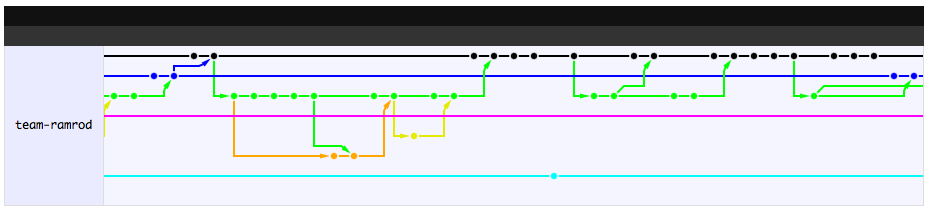
\includegraphics[width=\linewidth]{images/branching}
        \end{itemize}

      \end{frame}

    \subsection{Github}
      \begin{frame}{Github}
        \only<1>{
          \begin{block}{About}

            \emph{``Originally founded by Chris Wanstrath, PJ Hyett and Tom
            Preston-Werner as a project to simplify sharing code, GitHub has
            grown into an application used by nearly a million people to store
            over two million code repositories, making GitHub the largest code
            host in the world.''}~--~\url{https://github.com/about}

          \end{block}

        }
        \only<2>{
          \Huge \centering \scshape{Web Interface}\footnotemark[2]

          \vspace{0.5\baselineskip}
          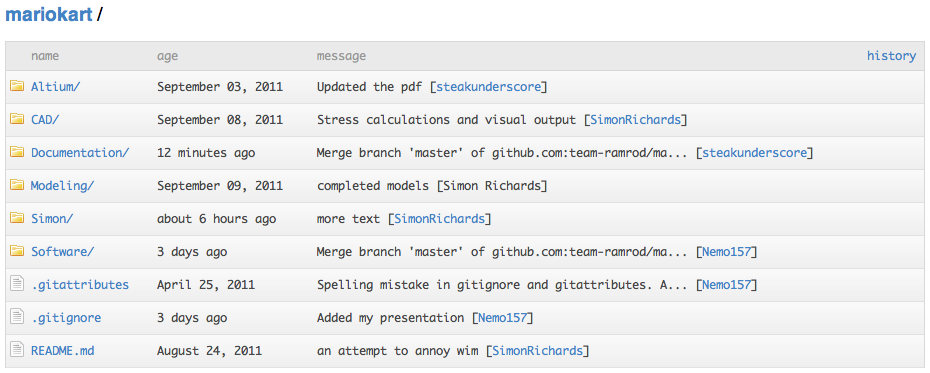
\includegraphics[width=\textwidth]{images/web-interface}

          \footnotetext[2]{\url{https://github.com/team-ramrod/mariokart}}
        }
        \only<3>{
          \Huge \centering \scshape{Wiki}\footnotemark[2]

          \vspace{0.5\baselineskip}
          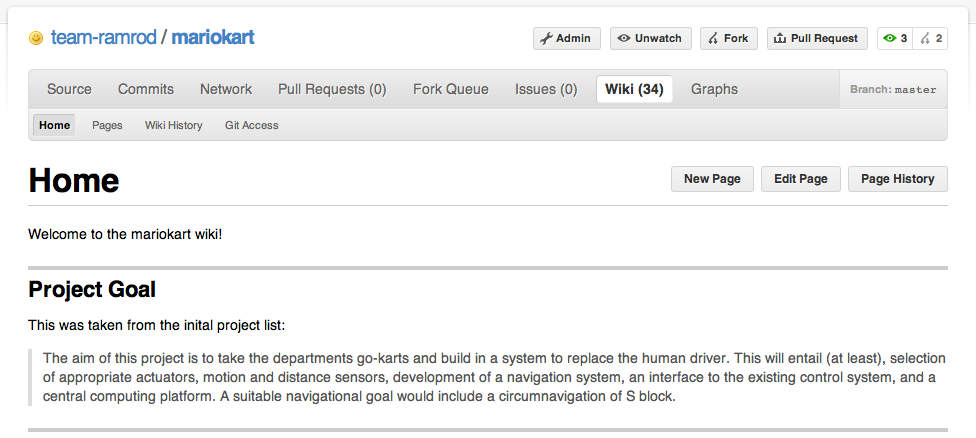
\includegraphics[width=\textwidth]{images/wiki}

          \footnotetext[2]{\url{https://github.com/team-ramrod/mariokart/wiki}}
        }
      \end{frame}

  \section{Continuous Integration}
    \subsection{What is it?}
      \begin{frame}{What Is Continuous Integration?}
        \begin{center}\begin{minipage}{0.8\linewidth}\begin{block}{Definition\footnotemark[2]}

              \emph{``Continuous Integration is a software development
              practice~\dots\ leading to multiple integrations per day~\dots\
              verified by an automated build~\dots\ to detect integration errors
              as quickly as possible.''}~---~Martin Fowler

        \end{block}\end{minipage}\end{center}

        \footnotetext[2]{\url{http://martinfowler.com/articles/continuousIntegration.html}}
      \end{frame}

    \subsection{Why would you use it?}
      \begin{frame}{Why Would You Use Continuous Integration?}
        \Large
        \begin{itemize}
          \pause\item Detect errors early.
          \vspace{\baselineskip}
          \pause\item Minimizes time between error introduction and fix.
          \vspace{\baselineskip}
          \pause\item Provides a stable base for future work.
          \begin{itemize}
            \pause \item \large Very useful for branch-happy development in git.
          \end{itemize}
          \vspace{0.5\baselineskip}
          \pause\item Peer pressure
                
\includegraphics[height=11pt]{images/smiley-devil}.
        \end{itemize}
      \end{frame}

    \subsection{CI Joe}
      \begin{frame}{CI Joe\footnotemark[2]}
        \only<1>{
          \begin{center}\begin{minipage}{0.65\linewidth}\begin{block}{Repository Description}
            \emph{``CI Joe is a fun Continuous Integration server.''}
          \end{block}\end{minipage}\end{center}
        }

        \only<2->{
          \begin{itemize}
            \Large
            \item<2-> Simple setup.
            \vspace{\baselineskip}
            \item<3-> Designed to work with git.
            \vspace{\baselineskip}
            \item<4-> Can trigger a build via a post-hook on github.
            \vspace{\baselineskip}
            \item<5-> Reports status via build-hook (used to send email).
          \end{itemize}
        }

        \footnotetext[2]{\url{https://github.com/defunkt/cijoe}}
      \end{frame}

    \subsection{Examples}
      \begin{frame}{Example 1}
        \only<1>{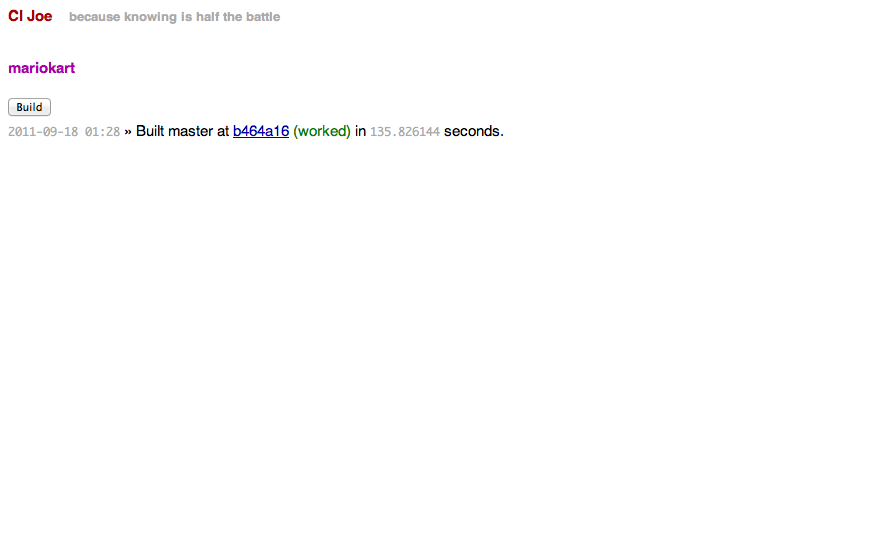
\includegraphics[width=\linewidth]{images/green-full}}
        \only<2>{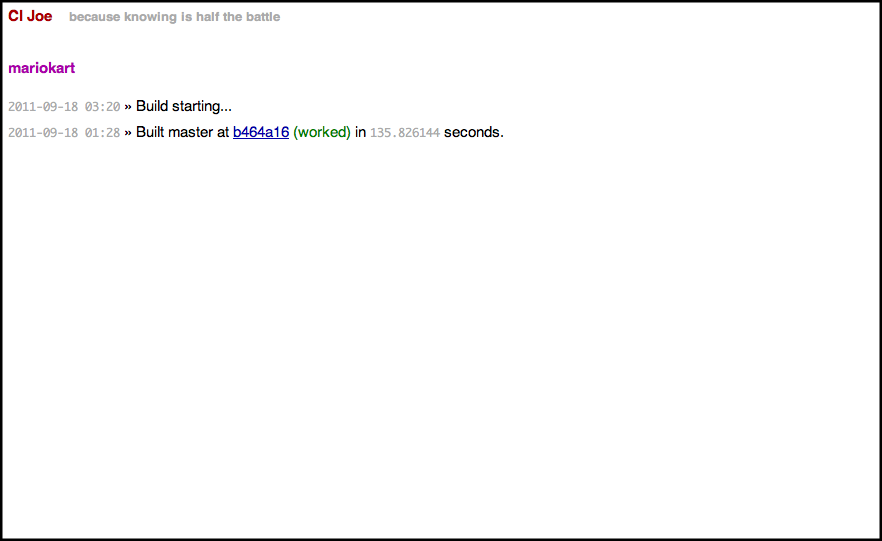
\includegraphics[width=\linewidth]{images/building-full}}
        \only<3>{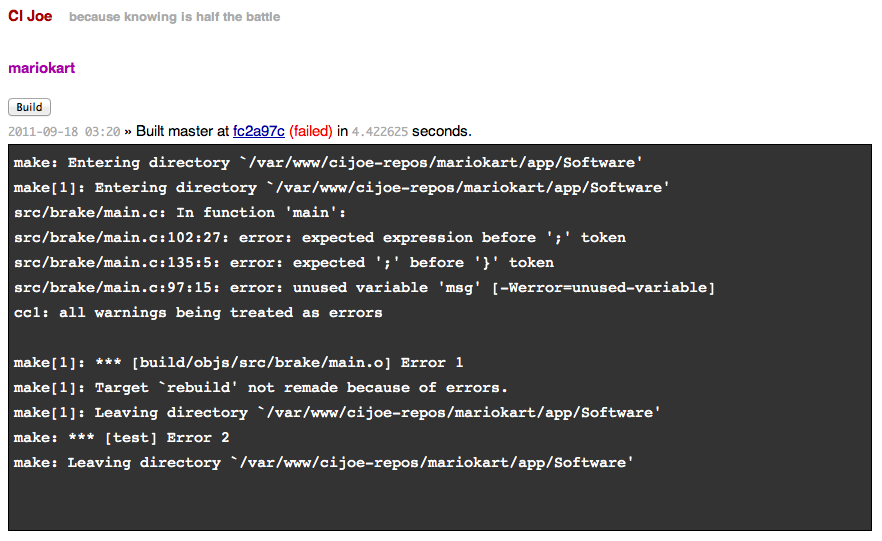
\includegraphics[width=\linewidth]{images/fail-full}}
      \end{frame}

      \begin{frame}{Example 2}
        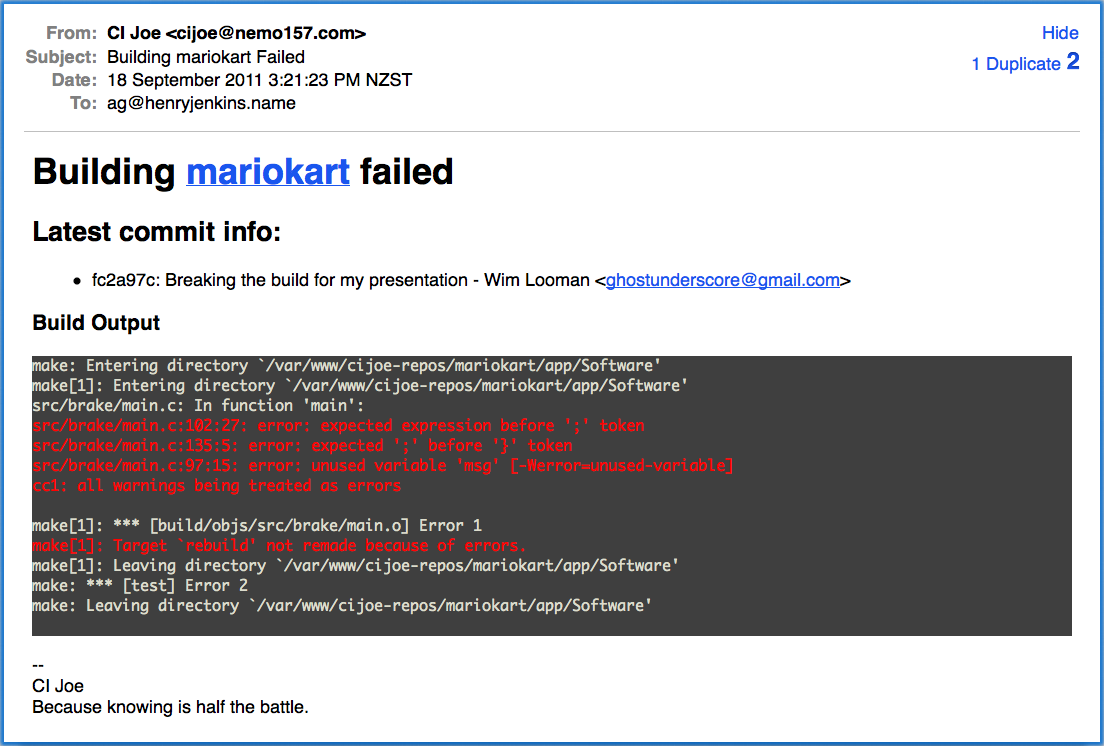
\includegraphics[width=\linewidth]{images/email}
      \end{frame}

    \section{Questions}
      \begin{frame}[plain]
        \begin{tikzpicture}[remember picture,overlay]
          \node[at=(current page.center)] {
            
\includegraphics[width=\paperwidth]{images/mario_kart_lego}
          };
        \end{tikzpicture}
      \end{frame}

    \begin{frame}{Git vs SVN}
      \begin{columns}
        \column{0.45\textwidth}
          \begin{block}{Git}
            \begin{itemize}
              \item Distributed (Generally used with a centralised repository).
              \item Every clone is a full repository.
              \item Nigh continual branching and merging is expected behaviour.
            \end{itemize}
          \end{block}

        \column{0.45\textwidth}
          \begin{block}{SVN}
            \begin{itemize}
              \item Needs a single central repository.
              \item Can't commit without access to central repository.
              \item Branching and merging is painful.
            \end{itemize}
          \end{block}
      \end{columns}
    \end{frame}

    \begin{frame}{Git Overview}
    \end{frame}

    \begin{frame}{Github Overview}
    \end{frame}

    \begin{frame}{Unit Testing}
      \begin{itemize}
        \item Initially was planned.
        \item Would require mocking the entire SAM7XC architecture.
        \begin{itemize}
          \item Hundreds to thousands of registers.
          \item Need constraints on which registers get written in which orders.
        \end{itemize}
        \item Would be awesome, but probably too large for even its own final year project.
      \end{itemize}
    \end{frame}
\end{document}
